Equations \eqref{eqn:eomx}, \eqref{eqn:eomy}, and \eqref{eqn:eomz} are our equations of motion that govern the movement of a satellite around a Lagrange point.
Technically, we can use them to represent motion anywhere in our system, not just around the Lagrange points.

Notice how the equations of motion are similar to \eqref{eqn:x-accel1}, where the distance, velocity, and acceleration of each dimension can not be represented separately as functions of time.
Still, it is possible to make use of these equations through numerical approximation.
This means that, given some initial conditions (position and velocity), the output is calculated (acceleration) for a small interval of time.
Than, after letting the new output determine the rest of the system for the said time interval, the output is recalculated with the given change from the initial conditions.
Recursively, this is generally written as:
\begin{equation*}
	y_{n+1} = y_n + hf(t_n)
\end{equation*}
where $h$ indicates the length of the time interval and where some value $y_0$ is known.
This particular equation is known as ``Euler's method''\autocite{BrilEulers} and is used to approximate equations that are similar to our equations of motion.
The method used to approximate the equations of motion will not specifically be Euler's method, but its purpose is practically identical.

$G$, $R$, and $\theta'$ are known constants, with the latter defined as:
\begin{equation*}
	\theta' = \omega = \sqrt{\frac{G(m_1 + m_2)}{R^3}} \text{,}
\end{equation*}
meaning the initial values are $x, y, z, x', y'$, and $z$.
By setting our initial $x$ coordinate $(1.511\times10^{11} - 10^3)\si{\metre}$, $1000\si{\metre}$ away from of L2, and the remaining conditions $y, z, x', y', z' = 0$, we get the following trajectory for $m_3$:
\begin{figure}[H]
	\centering
	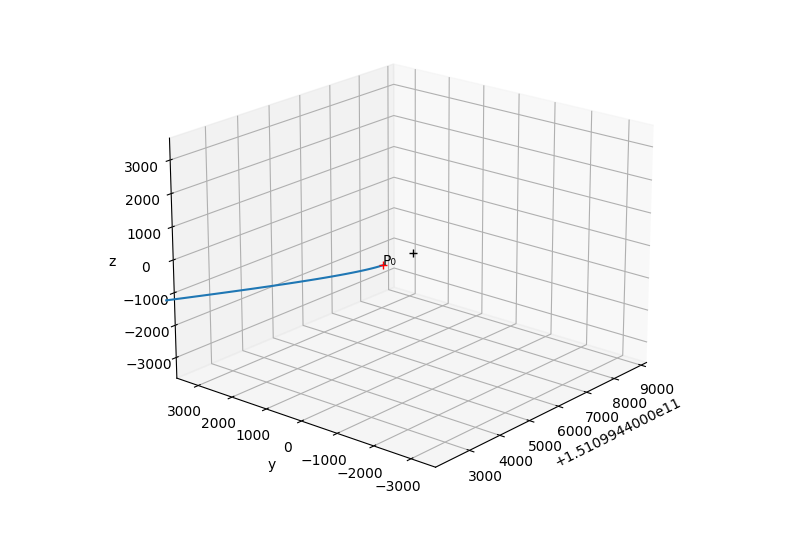
\includegraphics[scale=0.7]{3dplot1.png}
	\caption{Trajectory plot of an object near L2 fo the Sun-Earth system, x-coordinate is $(1.511\times10^{11} - 10^3)\si{\metre}$, all other conditions are 0. $P_0$ indicates the starting position of the object.}
	\label{fig:3dplot1}
\end{figure}
As seen in Figure \ref{fig:3dplot1}, the satellite unremarkably falls back towards the Earth.